% ================================================================
%  TimeVAE Weather Generation Experiment
%  Compile on Overleaf with pdfLaTeX
% ================================================================
\documentclass[aspectratio=169,10pt]{beamer}

% ---------- THEME ----------
\usetheme{Boadilla}
\usecolortheme{whale}
\setbeamertemplate{navigation symbols}{}
\setbeamertemplate{footline}{%
  \leavevmode%
  \hbox{%
    \begin{beamercolorbox}[wd=.65\paperwidth,ht=2.25ex,dp=1ex,leftskip=.3cm]%
        {author in head/foot}%
      \usebeamerfont{author in head/foot}%
      \insertshortauthor\quad|\quad\insertshorttitle
    \end{beamercolorbox}%
    \begin{beamercolorbox}[wd=.35\paperwidth,ht=2.25ex,dp=1ex,rightskip=.3cm,right]%
        {date in head/foot}%
      \usebeamerfont{date in head/foot}%
      \insertshortdate{}\quad
      \insertframenumber{} / \inserttotalframenumber
    \end{beamercolorbox}}%
  \vskip0pt}

% ---------- PACKAGES ----------
\usepackage{amsmath,amssymb,mathtools}
\usepackage{booktabs}
\usepackage{array}
\usepackage{xcolor}
\usepackage{colortbl}
\usepackage{tikz}
\usetikzlibrary{arrows.meta,positioning}

% ---------- COLORS ----------
\definecolor{myblue}{RGB}{31,119,180}
\definecolor{myred}{RGB}{180,30,30}
\definecolor{mygreen}{RGB}{30,130,30}
\definecolor{mygray}{RGB}{110,110,110}
\definecolor{boxblue}{RGB}{210,228,252}
\definecolor{boxyellow}{RGB}{255,250,200}
\definecolor{boxgreen}{RGB}{210,245,210}

% ---------- TITLE ----------
\title[TimeVAE Weather Generation]{%
  TimeVAE for Weather Time-Series Generation}
\subtitle{Experiment Definition, HPO, Loss Design, and Evaluation}
\author[Jinyu Li]{Jinyu Li}
\institute[UCL]{University College London}
\date[May 2026]{May 2026}

% ================================================================
\begin{document}
% ================================================================

\begin{frame}
  \titlepage
\end{frame}

\begin{frame}{Outline}
  \tableofcontents
\end{frame}

% ================================================================
\section{Experiment Definition}
% ================================================================

\begin{frame}{Task: What Generates What?}
  \begin{columns}[T]
    \column{0.52\textwidth}
      \textbf{Observed weather windows}
      \[
        \mathbf{X}_{c,i}\in\mathbb{R}^{T\times D},
        \qquad T=84,\quad D=5
      \]
      \begin{itemize}
        \item $c\in\mathcal{C}$: city index
        \item $i$: sliding-window sample index
        \item Features:
          \[
            (z500,\ t850,\ t2m,\ u10,\ v10)
          \]
        \item Stored dataset shape per city:
          \[
            \mathbf{X}_{c}\in\mathbb{R}^{18909\times84\times5}
          \]
      \end{itemize}

    \column{0.48\textwidth}
      \textbf{Generation objective}
      \[
        q_{\theta,c}(\tilde{\mathbf{X}})
        \approx
        p_{\mathrm{data},c}(\mathbf{X})
      \]
      \begin{itemize}
        \item Train one TimeVAE distribution model per city.
        \item Generate synthetic windows
          $\tilde{\mathbf{X}}_{c,j}\in\mathbb{R}^{84\times5}$.
        \item Goal: preserve multivariate weather-window distribution,
              not forecast the next value directly.
      \end{itemize}
      \begin{block}{City set}
        \small
        Cape Town, Hong Kong, London, New York, Singapore.
      \end{block}
  \end{columns}
\end{frame}

\begin{frame}{Data Split and Notation}
  \textbf{Full span used in this experiment:} 2003--2015.

  \vspace{0.5em}
  \begin{columns}[T]
    \column{0.50\textwidth}
      \textbf{Training split}
      \[
        \mathcal{D}^{\mathrm{train}}_c
        =
        \left\{
          \mathbf{X}_{c,i}\in\mathbb{R}^{84\times5}
          : \mathrm{time}(\mathbf{X}_{c,i})\subseteq
          [2003,2013]
        \right\}
      \]
      \begin{itemize}
        \item Used to fit TimeVAE parameters $\theta_c$.
        \item Scaler fitted on training windows only.
      \end{itemize}

    \column{0.50\textwidth}
      \textbf{Validation split}
      \[
        \mathcal{D}^{\mathrm{val}}_c
        =
        \left\{
          \mathbf{X}_{c,i}\in\mathbb{R}^{84\times5}
          : \mathrm{time}(\mathbf{X}_{c,i})\subseteq
          [2014,2015]
        \right\}
      \]
      \begin{itemize}
        \item Used for HPO selection and early stopping.
        \item Best HPO per city minimizes validation loss.
      \end{itemize}
  \end{columns}

  \vspace{0.5em}
  \begin{alertblock}{Generated data}
    \small
    After HPO, sample latent vectors
    $\mathbf{z}\sim\mathcal{N}(\mathbf{0},\mathbf{I})$ and decode
    $\tilde{\mathbf{X}}=g_{\theta_c}(\mathbf{z})$.
  \end{alertblock}
\end{frame}

% ================================================================
\section{HPO Setup}
% ================================================================

\begin{frame}{Hyperparameter Optimization}
  \begin{columns}[T]
    \column{0.52\textwidth}
      \textbf{Grid search per city}
      \[
        2\times4\times3\times3 = 72
        \quad\text{runs per city}
      \]
      \vspace{0.2em}

      \begin{tabular}{@{}ll@{}}
        \toprule
        Hyperparameter & Search values \\
        \midrule
        Latent dimension $d_z$ & $\{8,\ 16\}$ \\
        Reconstruction weight $\alpha$ & $\{0.01,\ 0.1,\ 1.0,\ 10.0\}$ \\
        Learning rate $\eta$ & $\{10^{-4},\ 10^{-3},\ 10^{-2}\}$ \\
        Batch size $B$ & $\{16,\ 32,\ 64\}$ \\
        \bottomrule
      \end{tabular}

    \column{0.48\textwidth}
      \textbf{Fixed settings}
      \begin{itemize}
        \item Model: TimeVAE.
        \item Encoder/decoder filters:
          \[
            [50,\ 100,\ 200]
          \]
        \item Optimizer: Adam.
        \item Maximum epochs: $1000$.
        \item Seed: $42$.
        \item Selection criterion:
          \[
            \arg\min_{\lambda\in\Lambda}
            \mathcal{L}_{\mathrm{val}}(\lambda;c)
          \]
      \end{itemize}
  \end{columns}
\end{frame}

% ================================================================
\section{Early Stopping}
% ================================================================

\begin{frame}{Early Stopping and Checkpoint Selection}
  \begin{columns}[T]
    \column{0.54\textwidth}
      \textbf{Monitor}
      \[
        m_e = \mathcal{L}_{\mathrm{val}}^{(e)}
        =
        \mathrm{MSE}_{\mathrm{val}}^{(e)}
        +
        \mathrm{KL}_{\mathrm{val}}^{(e)}
      \]
      \begin{itemize}
        \item Monitor validation total loss when validation data exist.
        \item Minimize mode.
        \item Minimum improvement:
          \[
            \Delta_{\min}=10^{-4}
          \]
        \item Patience:
          \[
            P=50\ \mathrm{epochs}
          \]
      \end{itemize}

    \column{0.46\textwidth}
      \textbf{Training control}
      \begin{itemize}
        \item Early stopping starts after
          $e_{\mathrm{start}}$.
        \item Current runs use
          \[
            e_{\mathrm{start}}=0
          \]
          unless explicitly overridden.
        \item Best weights are restored at training end.
        \item Learning rate is reduced on plateau:
          factor $0.5$, patience $30$.
      \end{itemize}

      \begin{block}{Practical effect}
        \small
        Each HPO run reports the best epoch and the minimum
        validation total loss.
      \end{block}
  \end{columns}
\end{frame}

% ================================================================
\section{TimeVAE Loss}
% ================================================================

\begin{frame}{TimeVAE Loss: Original vs. Current}
  \begin{columns}[T]
    \column{0.50\textwidth}
      \textbf{Original TimeVAE-style objective}
      \[
        \mathcal{L}_{\mathrm{orig}}
        =
        \alpha\,
        \underbrace{
        \mathbb{E}\left[
          \lVert\mathbf{X}-\hat{\mathbf{X}}\rVert_2^2
        \right]}_{\mathcal{L}_{\mathrm{rec}}}
        +
        \underbrace{
        D_{\mathrm{KL}}
        \left(
          q_{\phi}(\mathbf{z}\mid\mathbf{X})
          \,\Vert\,
          p(\mathbf{z})
        \right)}_{\mathcal{L}_{\mathrm{KL}}}
      \]
      \begin{itemize}
        \item Fixed KL pressure from the beginning.
        \item Can encourage posterior collapse or unstable trade-offs.
      \end{itemize}

    \column{0.50\textwidth}
      \textbf{Current objective, inspired by Niels' note}
      \[
        \mathcal{L}_{\mathrm{train}}^{(e)}
        =
        \alpha\,\mathcal{L}_{\mathrm{rec}}
        +
        \beta_e
        \frac{1}{N}\sum_{i=1}^{N}\sum_{j=1}^{d_z}
        \max\left(
          \mathrm{KL}_{ij},\lambda_{\mathrm{fb}}
        \right)
      \]
      \[
        \beta_e=\min\left(1,\frac{e}{E_{\mathrm{anneal}}}\right),
        \qquad
        E_{\mathrm{anneal}}=50,\quad
        \lambda_{\mathrm{fb}}=0.1
      \]
      \begin{itemize}
        \item KL annealing: reconstruction first, regularization later.
        \item Free bits: each latent dimension keeps minimum capacity.
      \end{itemize}
  \end{columns}
\end{frame}

% ================================================================
\section{Generation Quality}
% ================================================================

\begin{frame}{Quality Evaluation: Fast Reliable First Pass}
  \begin{columns}[T]
    \column{0.50\textwidth}
      \textbf{Step 1: select generators}
      \begin{itemize}
        \item For each city, choose the best HPO configuration on
              $\mathcal{D}^{\mathrm{val}}_c$.
        \item Load the best checkpoint.
        \item Generate $M$ synthetic windows:
          \[
            \tilde{\mathbf{X}}_{c,1:M}
            =
            g_{\theta_c}
            \left(
              \mathbf{z}_{1:M}
            \right),
            \quad
            \mathbf{z}_j\sim\mathcal{N}(\mathbf{0},\mathbf{I})
          \]
      \end{itemize}

    \column{0.50\textwidth}
      \textbf{Step 2: evaluate on test set}
      \begin{itemize}
        \item Compare generated samples with held-out real windows.
        \item Fast metrics give a reliable screening before expensive
              downstream forecasting experiments.
        \item Candidate metric names from the reference paper:
          \begin{itemize}
            \item Discriminative score
            \item Predictive score
            \item Marginal distribution similarity
            \item Auto-correlation similarity
            \item Cross-correlation similarity
            \item Energy Distance
          \end{itemize}
      \end{itemize}
  \end{columns}
\end{frame}

\begin{frame}{Energy Distance as the First Metric}
  \textbf{Flatten each window for distribution comparison}
  \[
    \mathbf{x}_i=\mathrm{vec}(\mathbf{X}_i)\in\mathbb{R}^{TD},
    \qquad
    \tilde{\mathbf{x}}_j=\mathrm{vec}(\tilde{\mathbf{X}}_j)\in\mathbb{R}^{TD}
  \]

  \vspace{0.4em}
  Given real test samples
  $\{\mathbf{x}_i\}_{i=1}^{n}$
  and generated samples
  $\{\tilde{\mathbf{x}}_j\}_{j=1}^{m}$:
  \[
    \widehat{\mathcal{E}}^2
    =
    \frac{2}{nm}\sum_{i=1}^{n}\sum_{j=1}^{m}
    \lVert\mathbf{x}_i-\tilde{\mathbf{x}}_j\rVert_2
    -
    \frac{1}{n^2}\sum_{i=1}^{n}\sum_{i'=1}^{n}
    \lVert\mathbf{x}_i-\mathbf{x}_{i'}\rVert_2
    -
    \frac{1}{m^2}\sum_{j=1}^{m}\sum_{j'=1}^{m}
    \lVert\tilde{\mathbf{x}}_j-\tilde{\mathbf{x}}_{j'}\rVert_2
  \]

  \begin{alertblock}{Interpretation}
    \small
    Lower Energy Distance means the generated and real test-window
    distributions are closer. It is model-free, multivariate, and useful
    as the first fast screening metric.
  \end{alertblock}
\end{frame}

\begin{frame}{Quality Evaluation: Forecasting Utility}
  \begin{columns}[T]
    \column{0.52\textwidth}
      \textbf{Downstream protocol}
      \begin{itemize}
        \item Train forecasting models on real data only.
        \item Train the same models on real plus generated data.
        \item Compare held-out forecasting performance.
      \end{itemize}

      \vspace{0.2em}
      \[
        \mathrm{Gain}
        =
        \mathrm{Metric}
        \left(
          f_{\mathrm{real+synthetic}}
        \right)
        -
        \mathrm{Metric}
        \left(
          f_{\mathrm{real}}
        \right)
      \]

    \column{0.48\textwidth}
      \textbf{Forecasters}
      \begin{itemize}
        \item CrossFormer
        \item DeformTime
        \item Sonnet
      \end{itemize}

      \begin{block}{Compute note}
        \small
        This is the expensive evaluation path. It should follow the
        metric-based screening of best TimeVAE generators.
      \end{block}
  \end{columns}
\end{frame}

\begin{frame}{Experiment Roadmap}
  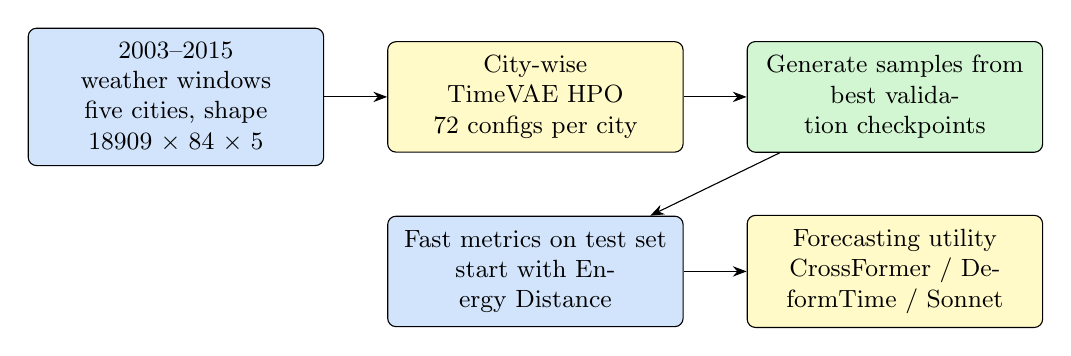
\begin{tikzpicture}[
      node distance=0.8cm,
      box/.style={draw, rounded corners=3pt,
                  text width=3.4cm, align=center,
                  font=\small, inner sep=5pt}]
    \node[box, fill=boxblue] (data) {2003--2015 weather windows\\
      five cities, shape $18909\times84\times5$};
    \node[box, fill=boxyellow, right=of data] (hpo) {City-wise TimeVAE HPO\\
      $72$ configs per city};
    \node[box, fill=boxgreen, right=of hpo] (gen) {Generate samples from\\
      best validation checkpoints};
    \node[box, fill=boxblue, below=of hpo] (metric) {Fast metrics on test set\\
      start with Energy Distance};
    \node[box, fill=boxyellow, right=of metric] (forecast) {Forecasting utility\\
      CrossFormer / DeformTime / Sonnet};

    \draw[-{Stealth[length=5pt]}] (data) -- (hpo);
    \draw[-{Stealth[length=5pt]}] (hpo) -- (gen);
    \draw[-{Stealth[length=5pt]}] (gen) -- (metric);
    \draw[-{Stealth[length=5pt]}] (metric) -- (forecast);
  \end{tikzpicture}
\end{frame}

% ================================================================
\end{document}
